

Homotopy theory is the study of spaces by way of their points, paths
(between points), homotopies (paths or continuous deformations between
paths), homotopies between homotopies (paths between paths between
paths), and so on.  This area of mathematics can be developed
\emph{synthetically} by using the homotopy-theoretic structure of types in
Martin-L\"of type
theory~\citep{hofmann98groupoid,lumsdaine09omega,vandenberggarner10groupoids,awodeywarren09identity,warren08thesis,gambinogarner08id,voevodsky11wollic}
to describe constructions in homotopy theory.  Using principles inspired
by these semantics, such such as higher inductive
types~\citep{lumsdaine+13hits,shulman11hitsblog,lumsdaine11hitsblog} and
Voevodsky's univalence
axiom~\citep{voevodsky11wollic,voevodsky+12simpluniv}, some aspects of
homotopy theory have been developed and formalized using the
Agda~\citep{norell07thesis} and Coq~\citep{inria06coqmanual} proof
assistants.  These include calculations of some homotopy groups of
spheres~\citep{ls13pi1s1,lb13pinsn,uf13hott-book}; constructions of the
Hopf fibration~\citep{uf13hott-book}, of covering
spaces~\citep{favonia-types}, and of Eilinberg-MacLane
spaces~\citep{lf14emspace}; and proofs of the Freudenthal suspension
theorem~\citep{uf13hott-book}, the Blakers-Massey theorem, the van
Kampen theorem~\citep{uf13hott-book}, and the Mayer-Vietoris
theorem~\citep{cavallo}.  Ideas from synthetic homotopy theory have also
been applied to represent the patch theories that arise in version
control systems using higher inductive types~\citep{amlh14patch}.

Many of the calculations, constructions, and proofs mentioned above were
posed as challenge problems during the 2012--2013 year on univalent
foundations at the Institute for Advanced Study.  One additional
challenge problem from that year, which was anticipated to be
\emph{less} difficult than those listed above, was
\begin{quote}
Show that the torus is equivalent to a product of two circles.
\end{quote}
In homotopy type theory, the elements of a type correspond to points of
a space, and the equality proofs in a type correspond to paths.  Using
higher inductive types, we describe a circle as being generated by a
point and a loop.  The picture
\begin{center}
  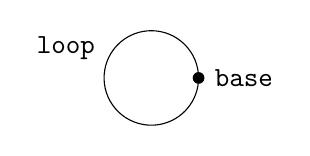
\begin{tikzpicture}
    \node[circle,fill,inner sep=1.5pt,label=right:{\texttt{base}}] (base) at (0,0) {};
    \draw (base) arc (0:170:.6cm) node[anchor=south east] {\texttt{loop}} arc (170:360:.6cm);
  \end{tikzpicture}
\end{center}
corresponds to a higher inductive type with one point constructor and
one path constructor:
\begin{verbatim}
base : S¹
loop : base == base
\end{verbatim}
(we write \verb|a == b| for the propositional equality/path type).
Similarly, we can describe a torus

[picture]

as a cell complex that consists of a square with opposite sides
identified:

This corresponds to the higher inductive type
\begin{verbatim}
a : T
p : a == a
q : a == a
f : q ∘ p == p ∘ q
\end{verbatim}
Algebraically, the torus is the free type with two loops that commute.

To prove that the torus is equivalent to the product of two circles
means to give functions \verb|t2c : T → S¹ × S¹| and
\verb|c2t : S¹ × S¹ → T| and show that they are mutually inverse (up to
propositional equality/paths).  At first glance, this task seems simple:
define the functions back and forth using the recursion principles for
the circle and the torus, and then prove that they are mutually inverse
using the induction principles for the circle and the torus.  And
indeed, it is not difficult to define the two functions.  However, at
the end of the IAS year, this problem had not been formalized in a proof
assistant, though Sojakova had given a proof sketch, which later
appeared as her heroic 25-page proof in the exercise solutions for the
homotopy type theory book~\citep{uf13hott-book}.  The reason for the
complexity is that the ``path algebra'' required to use the induction
principles to prove that the functions are mutually inverse gets quite
involved, because of the 2-dimensional ``face'' constructor \verb|f|.

In this paper, we develop a cubical approach to synthetic homotopy
theory.  With this approach, this motivating example of proving that the
torus is the product of two circles can be formalized in Agda in around
100 lines of code.  Moreover, this approach has proved useful for
several additional formalizations or programs: The second author used it
to formalize a ``three-by-three'' lemma about pushouts that is used in
the construction of the Hopf fibration.\footnote{URL} The first author
used it to prove a property of one of the patch theories that arose in
\citep{amlh14patch}\footnote{URL}.  Cavallo used it to simplify the
proof of the Mayer-Vietoris theorem~\citep{cavallo}.  In all of these
cases, the method simplifies constructions that were previously
difficult or intractable. 

Inspired by the cubical sets model of type
theory~\citep{coquand+13cubical}, the main idea of the approach is to
work with \emph{cube types} that generalize the path type \verb|a == b|.
For example, in this paper, we will consider a type of squares
\verb|Square l t b r|, dependent on four lines that fit into a square:
\begin{verbatim}
l : a00 == a01
r : a10 == a11
t : a00 == a10
b : a01 == a11
\end{verbatim}
[picture] and a type of cubes \verb|Cube left right front top bot back|
dependent on its six sides (as well as their boundaries).  Another
ingredient is to work systematically with ``path over a path'' and
``square over a square'' types, which represent paths and squares in a
fibration (dependent type).

While our approach fits nicely with work in progress on new cubical type
theories~\citep{us,altenkirchkaposi14cubical,coquand14variations}, the
present paper can be conducted entirely by making appropriate
definitions in Martin-L\"of type theory with univalence and higher
inductive types---no additional new axioms are needed.  Higher cubes can
be defined in terms of higher paths: for example, the type of squares
considered above can be thought of as discs \verb|b ∘ l == r ∘ t|.
Moreover, the notions of a ``path-over-a-path'' and a
``square-over-a-square'' can be reduced to homogeneous paths.  This
means that our constructions can be interpreted in the known models of
homotopy type theory with univalence and higher inductive
types~\cite{voevodsky+12simpluniv,shulman13inversediag,lumsdaine+13hits}.
While cubes can be reduced away in this way, for engineering reasons, we
have found it convenient in Agda to use new inductive families to
represent cube types; this allows us to make more effective use of
dependent pattern matching and unification.

First, we give a description of the cubical approach, including a survey
of a library (about 1500 lines of code) that contains the basic
definitions.  Then, we discuss the proof that the torus is equivalent to
a product of two circles.  

%%   In type theory, a space
%% corresponds to a type $A$. Points of a space correspond to elements $a,b
%% : A$. Paths in a space are modeled by elements of the identity type
%% (propositional equality), which we notate $p : a =_A b$.  Homotopies
%% between paths $p$ and $q$ correspond to elements of the iterated
%% identity type $p =_{a =_A b} q$.  The rules for the identity type allow
%% one to define the operations on paths that are considered in homotopy
%% theory.  These include identity paths $\dsd{id}_{a} : a = a$
%% (reflexivity of equality), inverse paths $\inv p : b = a$ when $p : a =
%% b$ (symmetry of equality), and composition of paths $q \comp p : a = c$
%% when $p : a = b$ and $q : b = c$ (transitivity of equality)\footnote{To
%%   match the Agda library used for our formalizations, we write path
%%   composition in function-composition order; this is different than in
%%   the Homotopy Type Theory book~\citep{uf13hott-book}.}, as well as
%% homotopies relating these operations (for example, $\dsd{id} \comp p =
%% p$), and homotopies relating these homotopies, etc.

